\chapter{Basic concepts}

%%%%%%%%%%%%%%%%%%%%%%%%%%%%%%%%%%%%%%%%%%%%%%%%%%%%%%%%%%%%%%%%%%%%%%%%%%%%%%%%%
\section{\textbf{\texttt{co2amp}} and \textbf{\texttt{co2amp+}}}
\textbf{\texttt{co2amp}} is a terminal program designed for simulating the propagation of ultrashort pulses through an arbitrary cylindrically-symmetric optical system, which may include \ce{CO2} amplifiers. It operates using inputs in the form of specially formatted text files and command line arguments, and generates outputs as tabulated data files and a binary file containing comprehensive information on the output field. While \textbf{\texttt{co2amp}} can function independently, its use is greatly facilitated by a graphical user interface, which significantly simplifies the management of the program’s inputs and outputs.

\textbf{\texttt{co2amp+}} is a graphical user interface program that streamlines the process of handling multiple input and output files, as well as calculation parameters, by maintaining an organized and easily navigable working environment. \textbf{\texttt{co2amp+}} features functionality for saving and recalling the entire file structure of a project along with command line parameters in a single compressed '.co2' file.


%%%%%%%%%%%%%%%%%%%%%%%%%%%%%%%%%%%%%%%%%%%%%%%%%%%%%%%%%%%%%%%%%%%%%%%%%%%%%%%%%
\section{Projects}
The \textbf{\texttt{co2amp}} input parameters include the characteristics of the initial \texttt{pulse(s)}, the optical \texttt{layout} configuration, specifications for all \texttt{optics} used in the model (including laser amplifiers), and calculation parameters (e.g., calculation grid definition).

The temporal shape of the pulse and the beam profile at every element of the optical layout are saved and can be accessed in both graphical and tabulated-numerical representations.

All \textbf{\texttt{co2amp}} inputs and outputs for a certain model constitute a project.

\textbf{\texttt{co2amp+}} facilitates the storage of all inputs and outputs of the model, except for the output field, in a single compressed project file with a '.co2' extension. Complete pulse information (complex field at every node of the space-time calculation grid) at the system's output can be saved separately as a binary HDF5 file (with a '.pulse' extension) and used as an input for another project. An example of the input file structure of a '.co2' project accessed via the \textbf{\texttt{co2amp+}} interface is illustrated in Fig.~\ref{fig:gui-input}.

\begin{figure}[ht]
 \centering
 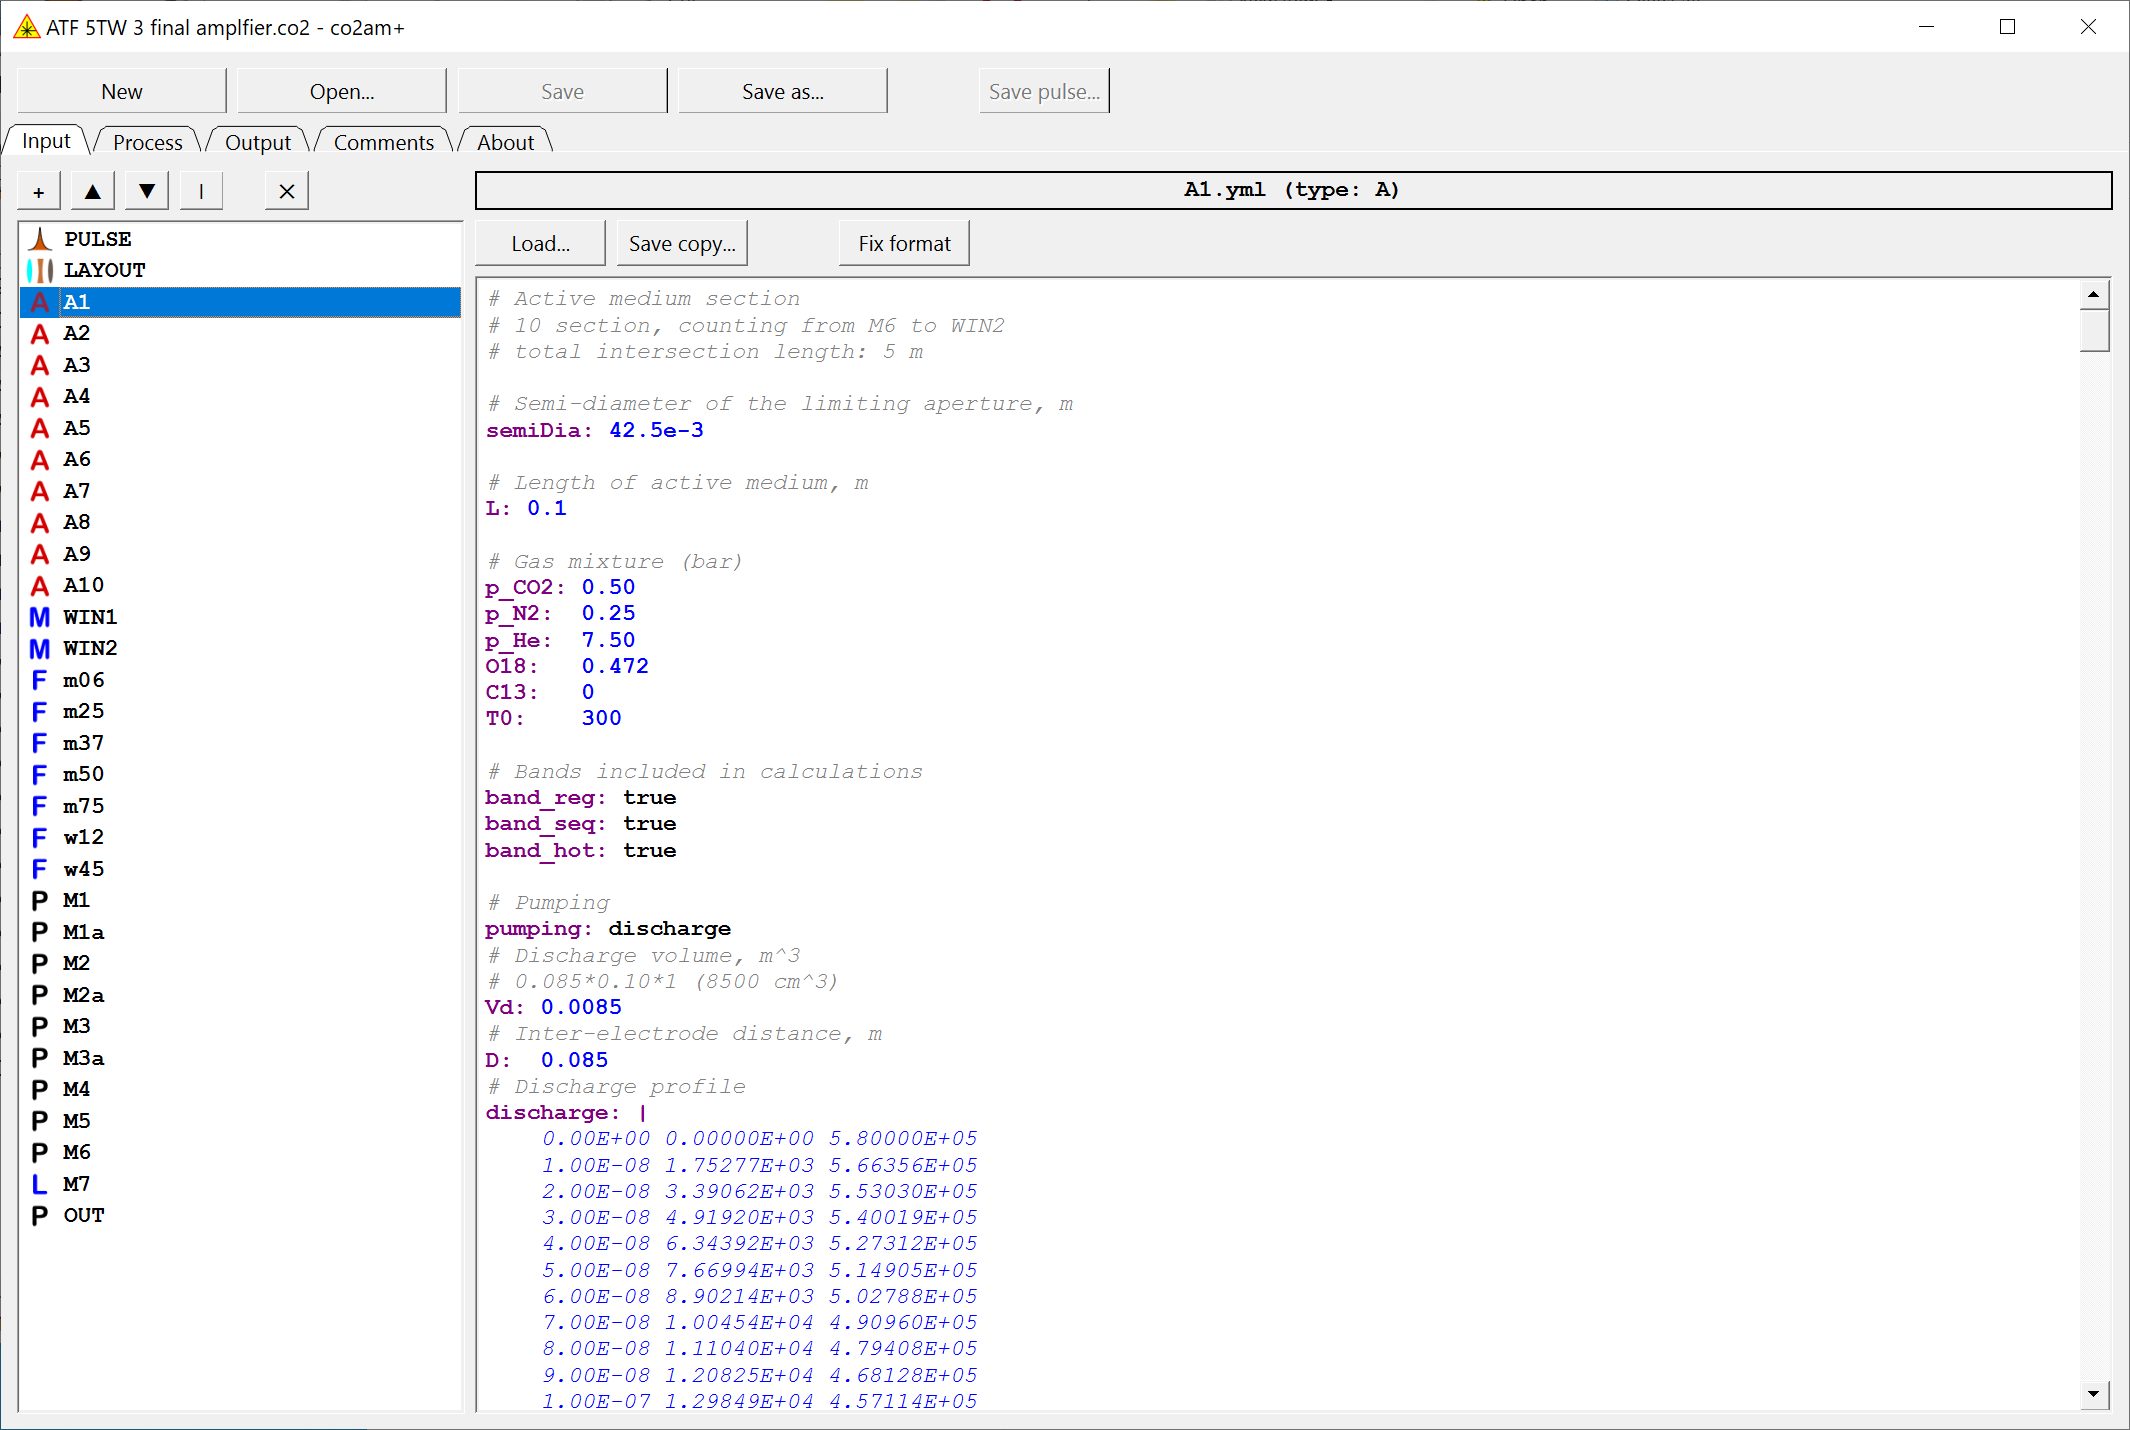
\includegraphics[width=14cm]{images/gui-input}
 \caption{"Input" tab of the \textbf{\texttt{co2amp+}} user interface program. YAML files specifying the \texttt{pulse}, \texttt{layout}, and \texttt{optics} are listed on the left. Content of a selected file is displayed and can be edited in the big edit box on the right.}
 \label{fig:gui-input}
\end{figure}


%%%%%%%%%%%%%%%%%%%%%%%%%%%%%%%%%%%%%%%%%%%%%%%%%%%%%%%%%%%%%%%%%%%%%%%%%%%%%%%%%
\section{\texttt{Pulse}, \texttt{Layout} and \texttt{Optic}}
A \texttt{pulse} is a complex electric field defined at every node of the calculation grid. A project can include one or more input pulses. Each is defined in a separate YAML ('.yml') file. A pulse can be defined either by referencing an output from another project (a '.pulse' file) or by explicitly specifying the pulse's spatial and temporal profile.

The optical \texttt{layout} consists of a series of infinitely-thin \texttt{optics} separated by free space. \texttt{Pulses} propagate freely between \texttt{optics}. A project must have exactly one \texttt{layout}. The \texttt{layout} is defined in a '.yml' file that specifies the order of the \texttt{planes} and the distances between them.

An \texttt{optic} is a system element that alters the pulse as it passes through. Several types of \texttt{optics} are described in detail later. For example, a \textit{Lens} is an \texttt{optic} introducing a radial-coordinate-dependent frequency shift, altering the beam's divergence. Each \texttt{optic} is specified in a separate '.yml' file. An \texttt{optic} can be used multiple times in the same \texttt{layout}, as in a laser cavity\footnote{Internally, the \textbf{\texttt{co2amp}} code employs an additional concept: a \texttt{plane}. A \texttt{plane} is a \texttt{layout} element that, unlike an \texttt{optic}, appears in the \texttt{layout} only once. An \texttt{optic} is then associated with each \texttt{plane}. Essentially, a \texttt{plane} is a placeholder for an \texttt{optic}.}.

\textbf{\texttt{co2amp}} supports seven types of \texttt{optics}, listed in Table~\ref{table:optics}.

\begin{table}
\caption{Types of \texttt{Optics}}
\label{table:optics}
\begin{tabularx}{\textwidth}{c l X}
\hline 
\textit{\textbf{Type ID}} & \textit{\textbf{Name}} & \textit{\textbf{Description}}\\
\hline 
&&\\
A & \textit{Active medium} & A CO$_2$ amplifier section.\\
&&\\
P & \textit{Probe} & A passive surface. May be used as a limiting aperture.\\
&&\\
F & \textit{Spatial filter} & An \texttt{optic} with coordinate-dependent transmission.\\
&&\\
S & \textit{Spectral filter} & An \texttt{optic} with frequency-dependent transmission.\\
&&\\
L & \textit{Lens} & An ideal thin lens.\\
&&\\
M & \textit{Material} & A layer of material. May introduce linear and/or non-linear dispersion and/or absorption.\\
&&\\
C & \textit{Chirper} & An \texttt{optic} that applies a chirp to the pulse. Typically a stretcher or compressor.\\
\hline
\end{tabularx}
\end{table}


%%%%%%%%%%%%%%%%%%%%%%%%%%%%%%%%%%%%%%%%%%%%%%%%%%%%%%%%%%%%%%%%%%%%%%%%%%%%%%%%%
\section{Calculation Grid}
The \texttt{pulse} is defined as a complex electric field at the nodes of a 2-dimensional space-time calculation grid, which moves with the pulse. The calculation grid is primarily defined via \textbf{\texttt{co2amp}} command line arguments. The only exception is the maximum radial coordinate, equal to the semi-diameter of the clear aperture of an \texttt{optic}, and thus varies from one \texttt{optic} to another. The command line arguments associated with the pulse's space-time calculation grid include the numbers of nodes (representing "precision") in the time and radial coordinate grids, the minimum and maximum time limits, and the central frequency. The central frequency is essential for unambiguously defining the calculation grid in the frequency domain.

The pulse time frame is utilized for all \texttt{pulse}-related calculations (interaction with \texttt{optics}, free-space propagation) and for fast processes in some \texttt{optics}, such as fast molecular dynamics (stimulated transitions and rotational relaxation in an \textit{Active Medium}). Processes significantly slower than the pulse duration (like the pumping of the active medium and vibrational relaxation) are modeled separately in a slower laboratory time-frame. The time-tick of this laboratory time-frame is also defined via a \textbf{\texttt{co2amp}} command line argument.

In \textbf{\texttt{co2amp+}}, the \textbf{\texttt{co2amp}} command line arguments are specified in the "Process" tab (Fig.~\ref{fig:gui-process}).
\begin{figure}[ht]
 \centering
 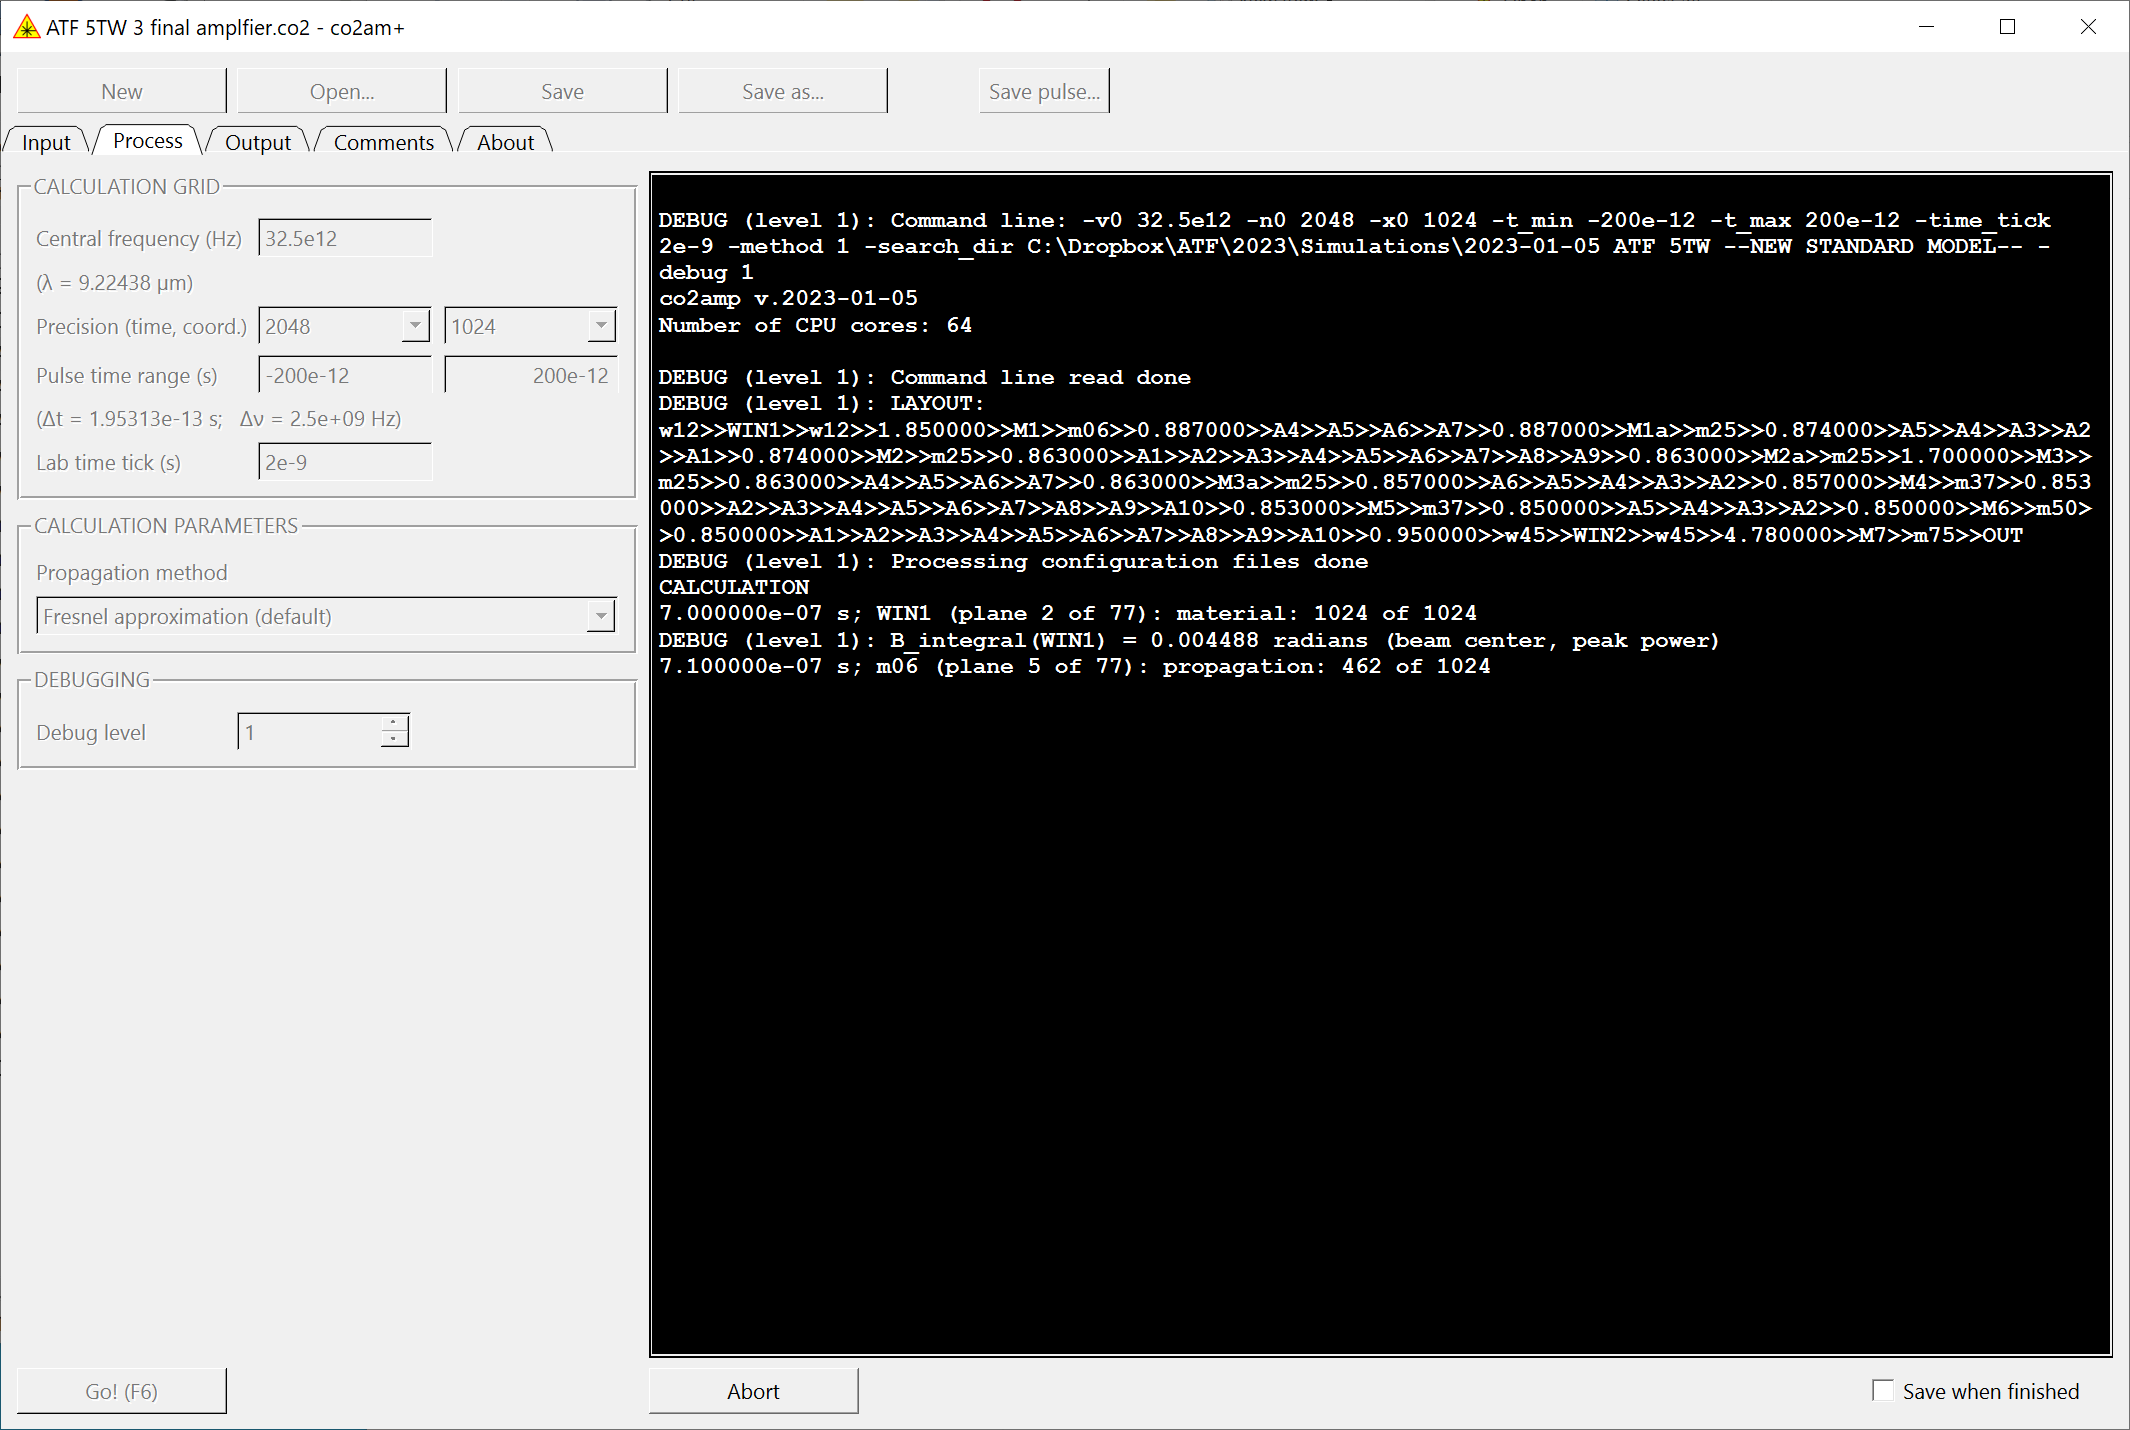
\includegraphics[width=14cm]{images/gui-process}
 \caption{"Process" tab of the \textbf{\texttt{co2amp+}} user interface program. Values of \textbf{\texttt{co2amp}} command line arguments are specified on the left. \textbf{\texttt{co2amp}} output is displayed in the black text box on the right.}
 \label{fig:gui-process}
\end{figure}
The number of nodes in both coordinates of the pulse space-time frame is always a power of two, enabling the use of Fast Fourier Transform (FFT) algorithms. Calculations with more nodes are generally more accurate but require longer computation times and more computer memory (both calculation time and required memory are approximately proportional to the product of the number of nodes in the time and space grids). Therefore, it is recommended to start the simulation with a smaller number of nodes and incrementally increase the grid density, repeating the simulation multiple times. The absence of significant changes in the program’s output with an increase in the number of nodes indicates that the grid density is satisfactory.

The time-step, \( \Delta t = (t_{\text{max}} - t_{\text{min}}) / N_t \), where \( t_{\text{max}} \) and \( t_{\text{min}} \) define the time range and \( N_t \) is the number of nodes in the time grid, must be sufficiently small to accurately describe the pulse profile throughout its propagation in the optical system. It is also important to note that the time range and the number of nodes in the time grid define the frequency domain range and step: \( \Delta\nu = 1 / (t_{\text{max}} - t_{\text{min}}) \) and \( (\nu_{\text{max}} - \nu_{\text{min}}) = 1 / \Delta t \). This means that the time range must be long enough to provide adequate resolution in the frequency domain, while the time step must be short enough to encompass the entire spectral region of interest.

Identifying an appropriate calculation grid is crucial for building an accurate model of an optical system. Investing effort in this part of the simulation process will yield fast and reliable calculations.


%%%%%%%%%%%%%%%%%%%%%%%%%%%%%%%%%%%%%%%%%%%%%%%%%%%%%%%%%%%%%%%%%%%%%%%%%%%%%%%%%
\section{Units}
SI units without prefixes, such as "meters, seconds, Amperes" (but not "centimeters, nanoseconds, kiloamperes"), are used in \textbf{\texttt{co2amp}} for input, output, and also internally within the code. \textbf{\texttt{co2amp+}} provides the functionality to change the units used for graphical representation of the calculation results on the "Output" tab (Fig.~\ref{fig:gui-output}).
\begin{figure}[ht]
 \centering
 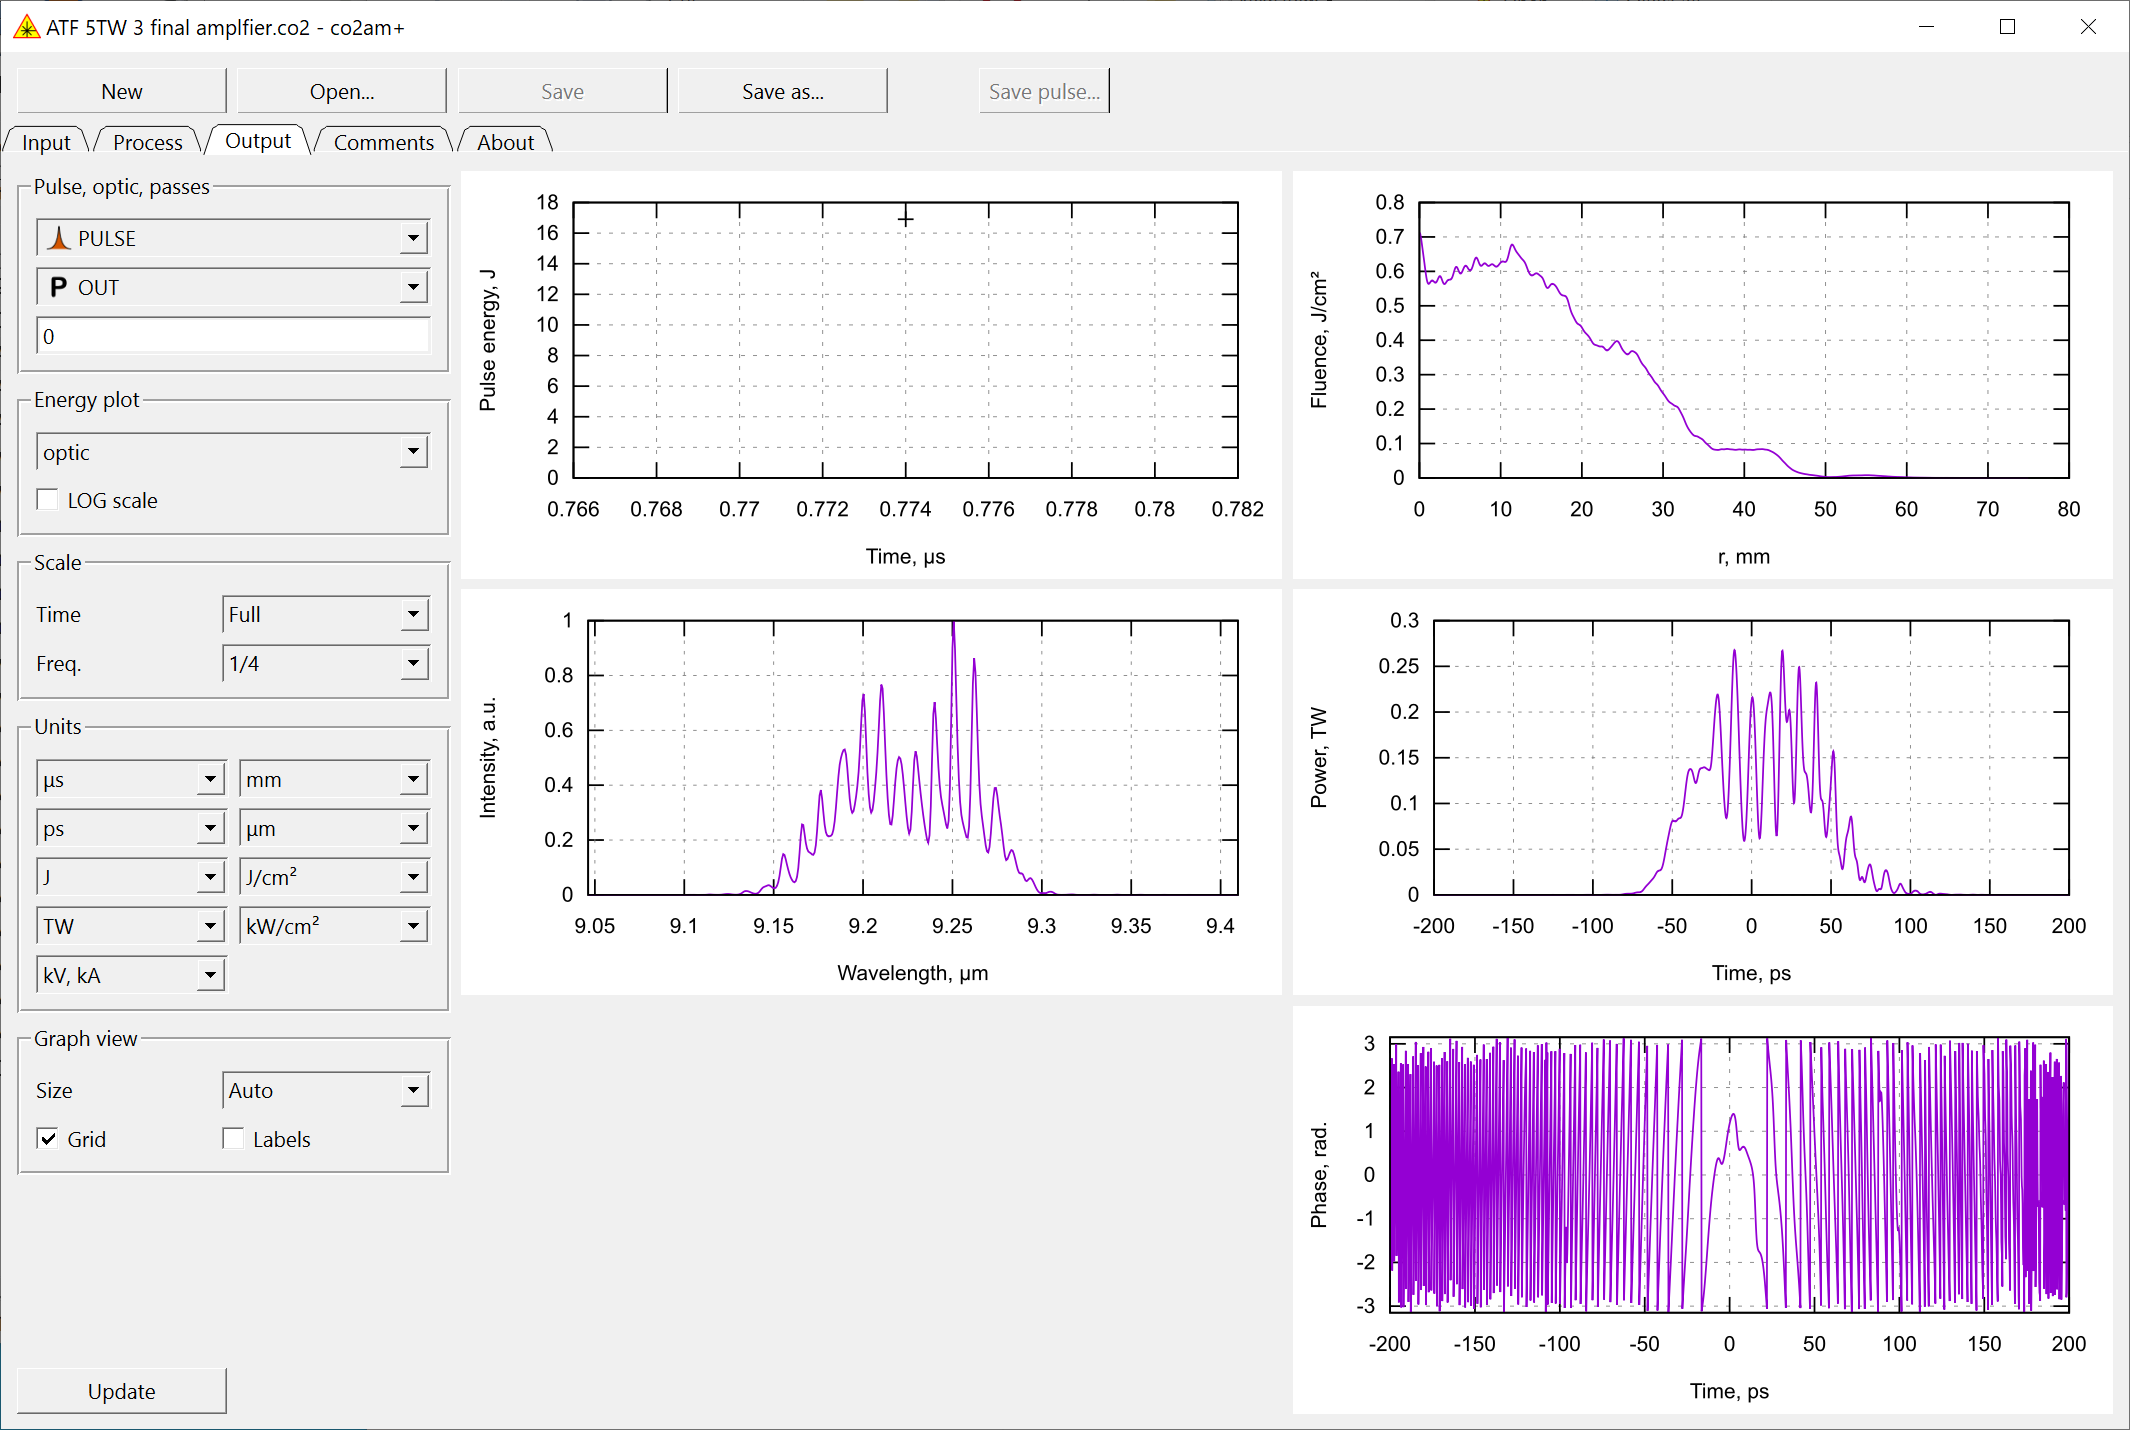
\includegraphics[width=14cm]{images/gui-output}
 \caption{"Output" tab of the \textbf{\texttt{co2amp+}} user interface program. Controls on the left allow selecting the data to display and fine-tuning the look of the plots.}
 \label{fig:gui-output}
\end{figure}
However, when numerical data are accessed via [Right-click on a plot] -- [Copy raw data], the units of the data are always in their "prefix-less" form.


%%%%%%%%%%%%%%%%%%%%%%%%%%%%%%%%%%%%%%%%%%%%%%%%%%%%%%%%%%%%%%%%%%%%%%%%%%%%%%%%%
\section{Program Output}
The output of the program includes the temporal and spatial structure of each \texttt{pulse} at every \texttt{optic} within the \texttt{layout}. Temporal (and spectral) profiles are integrated over the entire area of the \texttt{optic}, while spatial profiles are integrated over the duration of the pulse time-frame.

In the \textbf{\texttt{co2amp+}} "Output" tab, users can choose a \texttt{pulse} and an \texttt{optic} to display (Fig.~\ref{fig:gui-output}). If the selected \texttt{optic} is utilized multiple times in the \texttt{layout}, there is also an option to specify which passes through the \texttt{optic} are to be displayed. Additionally, the integral pulse energy can be provided either at each pass through a selected \texttt{optic} or across all passes through all \texttt{optics} in the \texttt{layout}.

Output for certain types of \texttt{optics} includes additional type-specific information. For example, for an \textit{Active medium}, this encompasses gain, discharge profile, population dynamics, and the dynamics of the distribution of pumping energy (fractions of discharge energy contributing to the excitation of laser levels, excitation of molecular translations, and ionization). Output for an \texttt{optic} of type \textit{Probe} includes information on the phase of the optical field at the center of the beam.


%%%%%%%%%%%%%%%%%%%%%%%%%%%%%%%%%%%%%%%%%%%%%%%%%%%%%%%%%%%%%%%%%%%%%%%%%%%%%%%%%
\section{"Comments" and "About" Tabs of \textbf{\texttt{co2amp+}}}
The "Comments" tab in \textbf{\texttt{co2amp+}} provides an editable text box where users can enter any comments about the project. These comments will be stored as part of the project in the '.co2' file.

The "About" tab contains information about the versions of \textbf{\texttt{co2amp}} and \textbf{\texttt{co2amp+}}, including links to the license and the documentation (this file), author contact information, and a suggested citation format.
